\section{Modellering}
I denne sektion vil der blive udarbejdet matematiske modeller for alle dele af systemet. Der vil være tale om et elektronisk system (motor og feedback), der er koblet til et mekanisk system (motorakslen, rammerne og den udveksling der forbinder dem). 

\subsection{Motor}
Motoren består af en rotor med flere XXXX poler, og en stator med en permanent magnet. Den permanente magnet sørger for at feltet, der påvirker rotoren, er nogenlunde konstant - dette forsimpler udregningen af motormomentet, da det er lineært afhængigt af magnetfeltet og strømmen igennem rotorvindingerne se ligning \ref{eq:motormoment}. Motorkonstanten $K_{m}$ er afhængig af permeabiliteten i det magnetiske materiale og kan bestemmes eksperimentielt - se reference her XXXX.

\begin{equation}\label{eq:motormoment}
T_{m}=K_{m}i_{a}(t)
\end{equation}

Den elektroniske del af motoren kan modelleres simpelt som en modstand $R_{a}$, som beskriver den samlede modstand i vindingerne, i serie med en spole $L_{a}$, som beskriver motorens induktans. Problemet med denne model er at den ikke tager højde for den modsatrettede spænding, der genereres i motorvindingerne, når rotoren er i bevægelse. Denne spænding er lineært afhængig af rotorens omdrejningshastighed og kan modelleres som en spændingskilde i serie med modstanden og spolen se figur \ref{fig:motor_sch}. $V_{b}=K_{e}\omega(t)$

\begin{wrapfigure}[15]{r}{0.4\textwidth}
\vspace{-20pt}
	\begin{center}
	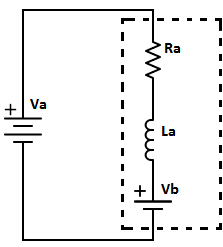
\includegraphics[scale=0.9]{Billeder/Motormodel.png}
	\end{center}
	\vspace{-10pt}
	\label{fig:motor_sch}
	\caption{Her ses et diagram af den omtalte motormodel}
\vspace{-20pt}
\end{wrapfigure}

Ved hjælp af Kirchoff's lov om spænding kan man nu udlede en differentialligning der relaterer alle elementerne efter spændingen over dem.

\begin{equation}\label{eq:DE_motor_1}
V_{a}=i(t)R_{a}+L_{a}\dfrac{di(t)}{dt}+K_{e}\omega(t)
\end{equation}

Den mekaniske del af motoren kan beskrives som det moment der genereres og driver en belastning. Momentet for enhver roterende masse kan beskrives ved Newton's 2. lov $T_{netto}=J\alpha(t)$, hvor $J$ er intertimomentet og $\alpha$ er vinkelaccelerationen. Denne ligning kan bruges til at beskrive nettomomentet for motoren og belastningen. 

\begin{equation}\label{eq:nettomoment}
T_{netto}=T_{m}-T_{f}
\end{equation}

Ligning \ref{eq:motormoment} kunne fortælle noget om momentet fra motoren, men det er også nødvendigt at have en dæmpende effekt i form a friktion med i modellen, for at den kan svare nogenlunde til virkeligheden. Heldigvis hænger det sådan sammen at det modsatrettede moment fra friktionen kan approksimeres ret præcist til at være lineært afhængigt af akslens omdrejningshastighed - denne linearitet kan beskrives ved $T_{f}=b\omega(t)$. Hvis man kombinerer alle tre ligninger ved at substituere dem ind i ligning \ref{eq:nettomoment}, er det muligt at danne endnu en differentialligning, der afhænger af rotoren's omdrejningshastighed.

\begin{equation}\label{DE_motor_2}
J\dfrac{d\omega(t)}{dt}=K_{m}i(t)-b\omega(t)
\end{equation}

Ligning \ref{eq:DE_motor_1} og \ref{DE_motor_2} kan tilsammen beskrive motoren og dens belastning ved at relatere spændingen over motorterminalerne til omdrejningshastigheden. Det er ydermere muligt at beregne sig frem til en vinkelposition- eller acceleration ved henholdsvis at integrere eller differentiere vinkelhastigheden.